\section{Sprint 2.2 : Finalisation et déploiement de l’application}
Ce sprint a permis de finaliser les fonctionnalités avancées et d’assurer la mise en production :
\begin{itemize}[label=$-$]
    \item \textbf{Gestion des scans multiples} : intégration des scans fonctionnels, sécurité et SEO dans une interface unifiée.
    \item \textbf{Visualisation des statistiques via le tableau de bord} : développement du tableau de bord pour un suivi clair des analyses.
    \item \textbf{Gestion des rapports des analyses effectuées} : mise en place des fonctionnalités de consultation et export des rapports.
    \item \textbf{Déploiement de l’application} : préparation et exécution du déploiement final en environnement de production.
\end{itemize}
Ce sprint a permis d’achever le projet en offrant une application complète et opérationnelle.

\subsection{Backlog du sprint 2.2}  
Dans cette section, nous présenterons le Backlog du sprint 2.2, illustré dans le tableau \ref{tab:backlogS22}, en tenant compte des modifications et ajustements apportés depuis le sprint précédent.
\begin{landscape}
    \renewcommand{\arraystretch}{1.1}
    \begin{spacing}{0.98}
        \begin{longtable}{|p{0.6cm}|p{3cm}|p{5.2cm}|p{1cm}|p{8.2cm}|p{0.6cm}|p{0.6cm}|p{1.2cm}|}
            \caption{Backlog du sprint 2.2} \label{tab:backlogS22} \\\hline
            \rowcolor{gray!20}
            \textbf{\small ID US} & 
            \multicolumn{1}{c|}{\textbf{\small User Story}} & 
            \multicolumn{1}{c|}{\textbf{\small Description}} & 
            \textbf{\small ID tâche}& 
            \multicolumn{1}{c|}{\textbf{\small Tâches}} & 
            \multicolumn{1}{c|}{\textbf{\small Priorité}} & 
            \multicolumn{1}{c|}{\textbf{\small Risques}} & 
            \textbf{\small Estim-ation(j)} \\\hline          
            % --- Gestion des analyses complètes (fonctionnels, sécurité, SEO) ------------
            \rowcolor{blue!20}
            \multicolumn{8}{|c|}{\textbf{EPIC 7 : Gestion des analyses complètes (fonctionnels, sécurité, SEO)}} \\\hline
            
            7.1 & Lancer plusieurs scans en parallèle selon le choix parmi les trois types de tests : fonctionnels, de sécurité et SEO. 
            & En tant que testeur, je dois pouvoir exécuter simultanément des tests fonctionnels, de sécurité et SEO pour gagner du temps et obtenir une analyse complète et globale.
            & 7.1.A \newline\vspace{0.5cm}7.1.B 
            & - Créer un interface et implémenter une logique permettant de choisir un ou plusieurs types de tests à exécuter (fonctionnel, sécurité, SEO) simultanément. \newline
              - Centraliser les résultats et générer un rapport unifié. \newline
            & Élevée & Élevée & 2 \\\hline
            
            7.2 & Consulter les résultats des différents types d’analyses de manière consolidée.
            & En tant que testeur, je souhaite consulter de manière centralisée les résultats fonctionnels, de sécurité et SEO afin de mieux comprendre les impacts croisés.
            & 7.2.A \newline 7.2.B
            & - Concevoir une interface unifiée pour la visualisation des résultats. \newline
              - Regrouper les vulnérabilités, erreurs fonctionnelles et recommandations SEO dans une vue consolidée.
            & Élevée & Moyenne & 2 \\\hline
            
            7.3 & Gérer les rapports d’analyse (suppression, export, recherche, relancement).
            & En tant qu'administrateur, je veux pouvoir rechercher, supprimer, exporter ou relancer un scan en utilisant la configuration d’un rapport existant pour faciliter la gestion des résultats.
            & 7.3.A \newline 7.3.B \newline 7.3.C
            & - Ajouter la possibilité de rechercher des rapports par mots-clés, type de test ou date. \newline
              - Permettre la suppression manuelle ou automatique des rapports. \newline
              - Intégrer une fonction d’export (PDF/JSON...). \newline
              - Offrir la possibilité de relancer un scan avec les paramètres d’un ancien rapport.
            & Moyenne & Moyenne & 2 \\\hline
           % ----------- Consultation des statistiques --------
            \rowcolor{blue!20}
            \multicolumn{8}{|c|}{\textbf{EPIC 8 : Visualisation des statistiques via le tableau de bord}} \\\hline
            
            8.1 & Visualiser des statistiques personnalisées des scans via le tableau de bord.
            & En tant que testeur, je souhaite suivre l'évolution de mes tests à travers un tableau de bord pour faciliter l’analyse.
            & 8.1.A \newline\vspace{0.5cm} 8.1.B
            & - Concevoir un tableau de bord interactif permettant d'afficher les résultats des scans. \newline
              - Représenter les statistiques personnelles sous forme graphique avec des filtres. 
            & Élevée & Moyenne & 4 \\\hline
            
            8.2 & Visualiser les statistiques globales via le tableau de bord administrateur.
            & En tant qu’administrateur, je souhaite disposer d’un tableau de bord centralisé pour superviser l’activité des utilisateurs, des scans et des autorisations.
            & 8.2.A \newline\vspace{0.5cm} 8.2.B
            & - Créer une interface d’administration affichant les statistiques globales : nombre de scans effectués, utilisateurs actifs, statuts des analyses... \newline
              - Ajouter des filtres dynamiques par période, gravité, type d’analyse, avec des représentations graphiques.
            & Moyenne & Moyenne & 4 \\\hline
            
            % ----------- EPIC 12 -----------------
            \rowcolor{blue!20}
            \multicolumn{8}{|c|}{\textbf{EPIC 12 : Gestion des rapports des analyses effectuées}} \\\hline

            12.1 & Consulter tous les rapports générés.
            & En tant qu’administrateur, je souhaite accéder à tous les rapports générés par les utilisateurs.
            & 12.1.A \newline 12.1.B
            & - Créer une interface d’affichage de rapports filtrables par type, date, utilisateur. \newline
              - Ajouter une fonction de recherche.
            & Moyenne & Basse & 1 \\\hline

            12.2 & Télécharger et supprimer les rapports.
            & En tant qu’administrateur, je souhaite pouvoir télécharger ou supprimer les rapports.
            & 12.2.A \newline 12.2.B
            & - Ajouter les options de téléchargement dans différents formats (HTML, JSON, PDF...). \newline
              - Implémenter la suppression sécurisée des rapports obsolètes.
            & Moyenne & Moyenne & 2 \\\hline

            % ----------- EPIC 13 -----------------
            \rowcolor{blue!20}
            \multicolumn{8}{|c|}{\textbf{EPIC 13 : Déploiement de l’application}} \\\hline
            
            13.1 & Conteneuriser les composants de l'application.
            & En tant que développeur, je souhaite conteneuriser les différentes parties de l’application pour en faciliter le déploiement, la portabilité et la maintenance.
            & 13.1.A \newline\vspace{1cm} 13.1.B
            & 
            – Conteneuriser les composants de l’application (PostgreSQL, backend FastAPI, frontend Angular, RabbitMQ) en créant des images Docker personnalisées, et intégrer les outils de sécurité (ZAP, SQLMap, Nuclei) dans des conteneurs dédiés. \newline
            – Préparer les fichiers Dockerfile avec les configurations pour chaque service.
            & Élevée & Moyenne & 2 \\\hline
            
            13.2 & Orchestrer les conteneurs avec Docker Compose.
            & En tant que développeur, je souhaite orchestrer le déploiement de tous les services à l’aide de Docker Compose pour assurer une configuration cohérente.
            & 13.2.A \newline\vspace{1cm} 13.2.B
            & 
            – Rédiger un fichier `docker-compose.yml` regroupant tous les services. \newline
            – Configurer les volumes partagés, les réseaux et les dépendances entre les conteneurs, puis vérifier leur communication et assurer le bon démarrage de l’ensemble.
            & Moyenne & Moyenne & 3 \\\hline
            
            \rowcolor{gray!20}
			\multicolumn{7}{|c|}{TOTAL} &  22UE \\
            \hline 
        \end{longtable}
    \end{spacing}
\end{landscape}

\subsection{Analyse du sprint 2.2}
Dans cette section, nous analysons les besoins fonctionnels couverts durant le sprint 2.2.
\subsubsection{Diagramme de cas d’utilisation du sprint 2.2}
Cette section présente le diagramme de cas d’utilisation élaboré pour le sprint 2.2, illustré dans la figure \ref{fig:caseS22}. Il met en évidence les différentes interactions entre les utilisateurs et le système, notamment l’exécution simultanée des analyses (fonctionnelles, de sécurité et SEO), la gestion des rapports par l’administrateur, ainsi que la visualisation des statistiques via le tableau de bord.
\begin{figure}[H]
    \centering
    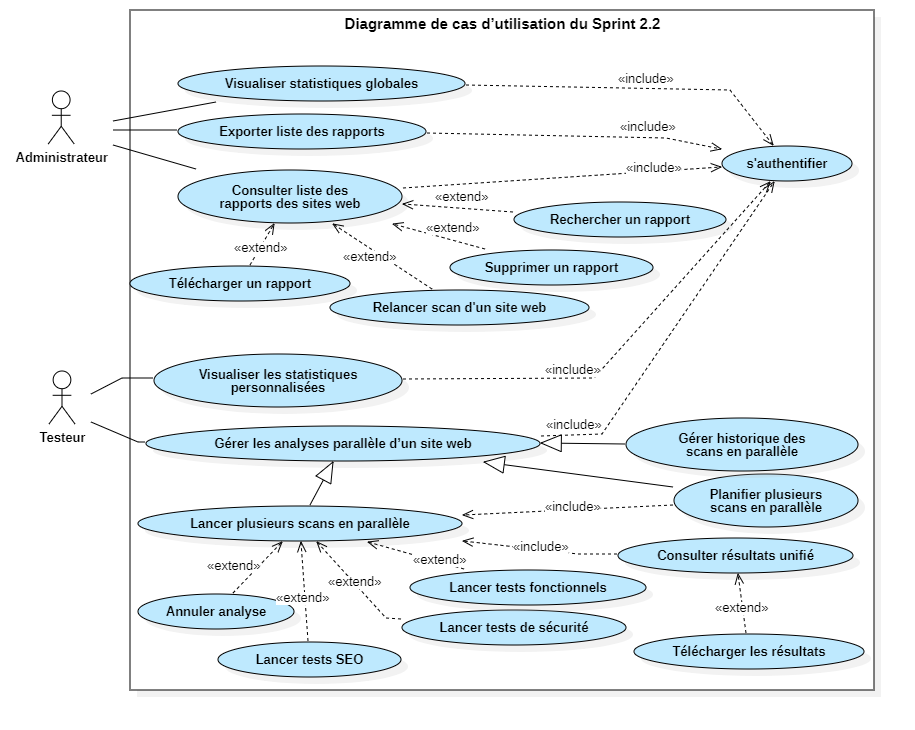
\includegraphics[width=\linewidth]{chapitres/ch4Sp2/section/sprint2.2/img/LastUseCaseSprint2.2.png}
    \caption{Diagramme de cas d'utilisation du sprint 2.2}
    \label{fig:caseS22}
\end{figure}
\vspace{-0.3cm}



\subsection{Conception du sprint 2.2}
Dans cette section, nous détaillons la conception des fonctionnalités développées au cours du sprint 2.2.

\subsection{Réalisation du sprint 2.2}
\begin{justify}
Dans cette section, nous présentons les principales interfaces développées durant cette sprint 2.2, en commençant par celles liées à l'exécution parallèle des tests, la gestion des rapports, puis la visualisation des statistiques.
\end{justify}
\begin{itemize}[label=$\bullet$]
    \item \textbf{Interface de la sélection des tests à exécuter} :  
    La figure \ref{fig:multiScanUI}\footnote{Voir annexe E : Figure \ref{fig:multiScanUI}} illustre l’interface permettant à l’utilisateur de sélectionner un ou plusieurs types d’analyses à effectuer (fonctionnelle, sécurité, SEO). Cette interface a été conçue pour offrir une interaction simple et efficace, favorisant l’exécution parallèle des différents scans.

    \item \textbf{Interface de visualisation consolidée des résultats} :  
    La figure \ref{fig:resultView}\footnote{Voir annexe E : Figure \ref{fig:resultView}} présente la vue unifiée des résultats d’analyse. Elle regroupe les vulnérabilités de sécurité, les erreurs fonctionnelles et les recommandations SEO dans une seule interface pour faciliter la lecture croisée et la prise de décision.

    \item \textbf{Interface de gestion des rapports d’analyse} :  
    Comme illustré dans la figure \ref{fig:reportManagementUI}, cette interface permet à l’administrateur de rechercher, supprimer, exporter les rapports. Les filtres intégrés (type, date, utilisateur) rendent la gestion des rapports plus fluide et performante.
    \begin{figure}
        \centering
        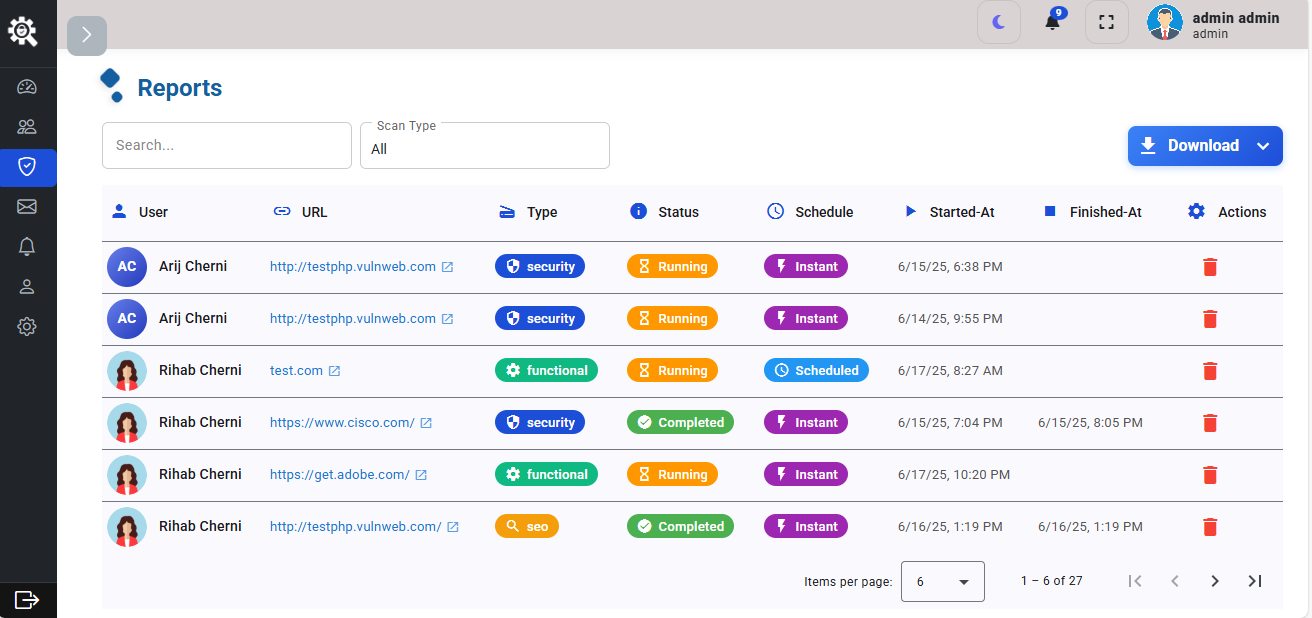
\includegraphics[width=\linewidth]{chapitres/ch4Sp2/section/sprint2.2/img/interface/reports-admin-liste.PNG}
        \caption{Caption}
        \label{fig:enter-label}
    \end{figure}

   \item \textbf{Tableau de bord utilisateur} :   La figure \ref{fig:testerdashboardUI}présente le tableau de bord dédié aux testeurs. Il affiche  des statistiques filtrables et interactives sur les campagnes de test, à travers des graphiques dynamiques.
    \begin{figure}[H]
        \centering
        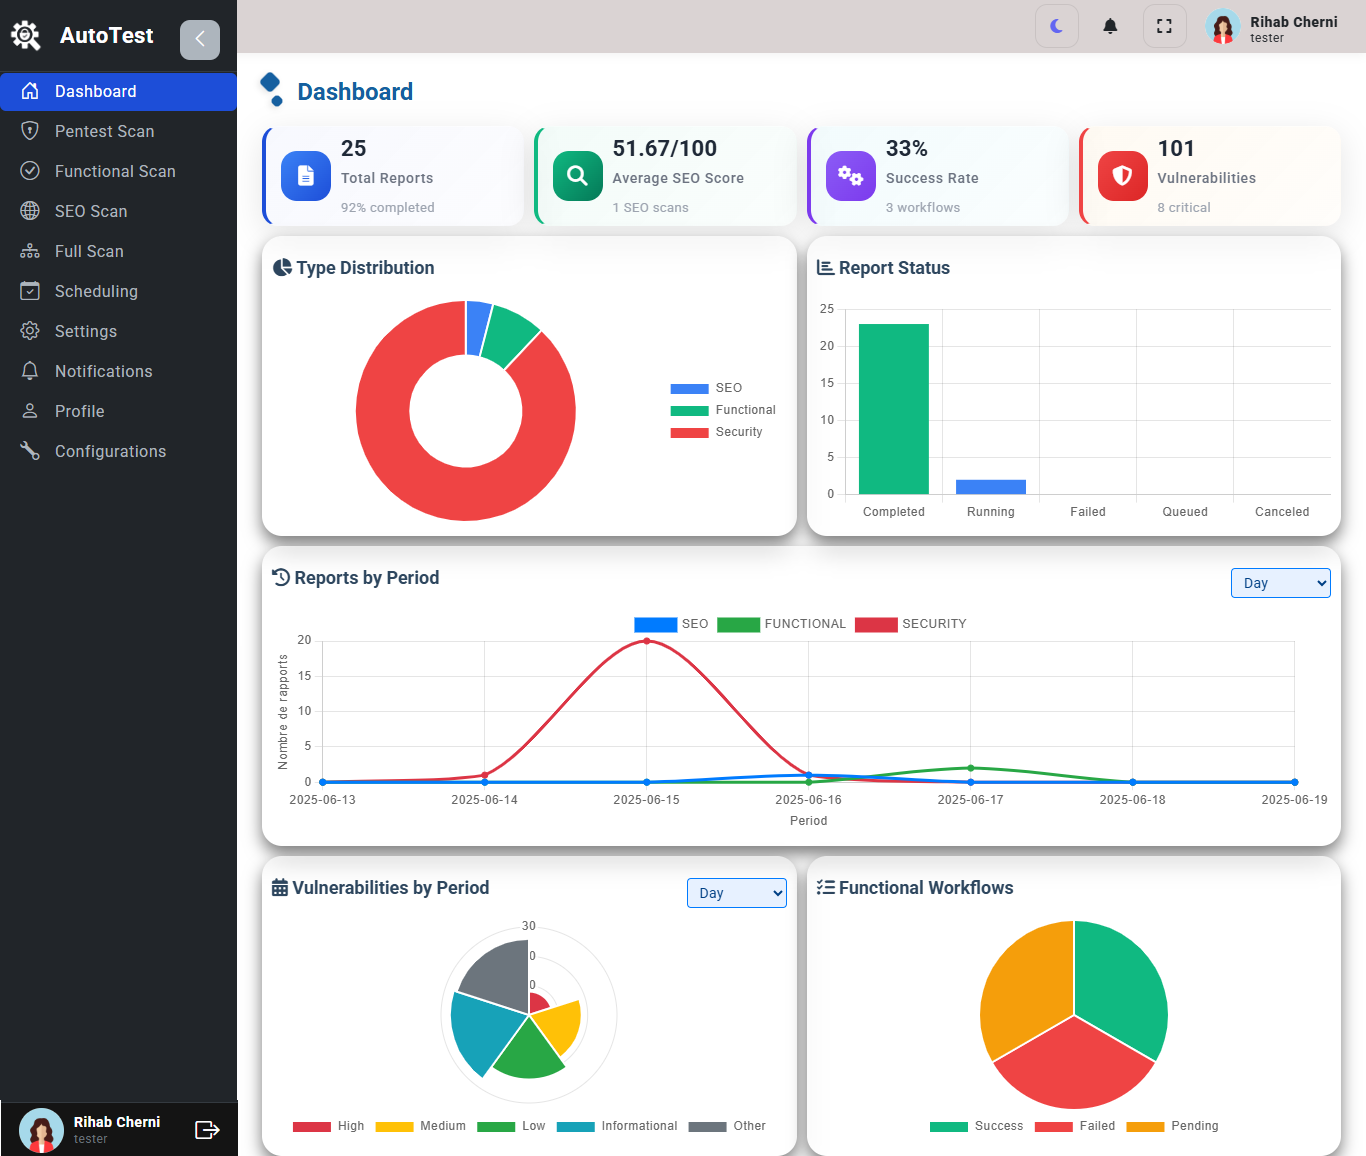
\includegraphics[width=\linewidth]{chapitres/ch4Sp2/section/sprint2.2/img/interface/tester-dashbaord.png}
        \caption{\centering Interface du tableau de bord testeur}
        \label{fig:testerdashboardUI}
    \end{figure}
    \vspace{-0.3cm}
    \item \textbf{Tableau de bord administrateur} :  
    Pour le profil administrateur, la figure \ref{fig:adminDashboardUI} met en évidence les indicateurs globaux sur l'activité de la plateforme : nombre de scans, utilisateurs actifs, types d’analyses effectuées, etc. Des filtres par période ou type d’analyse sont également disponibles.
    \begin{figure}[H]
        \centering
        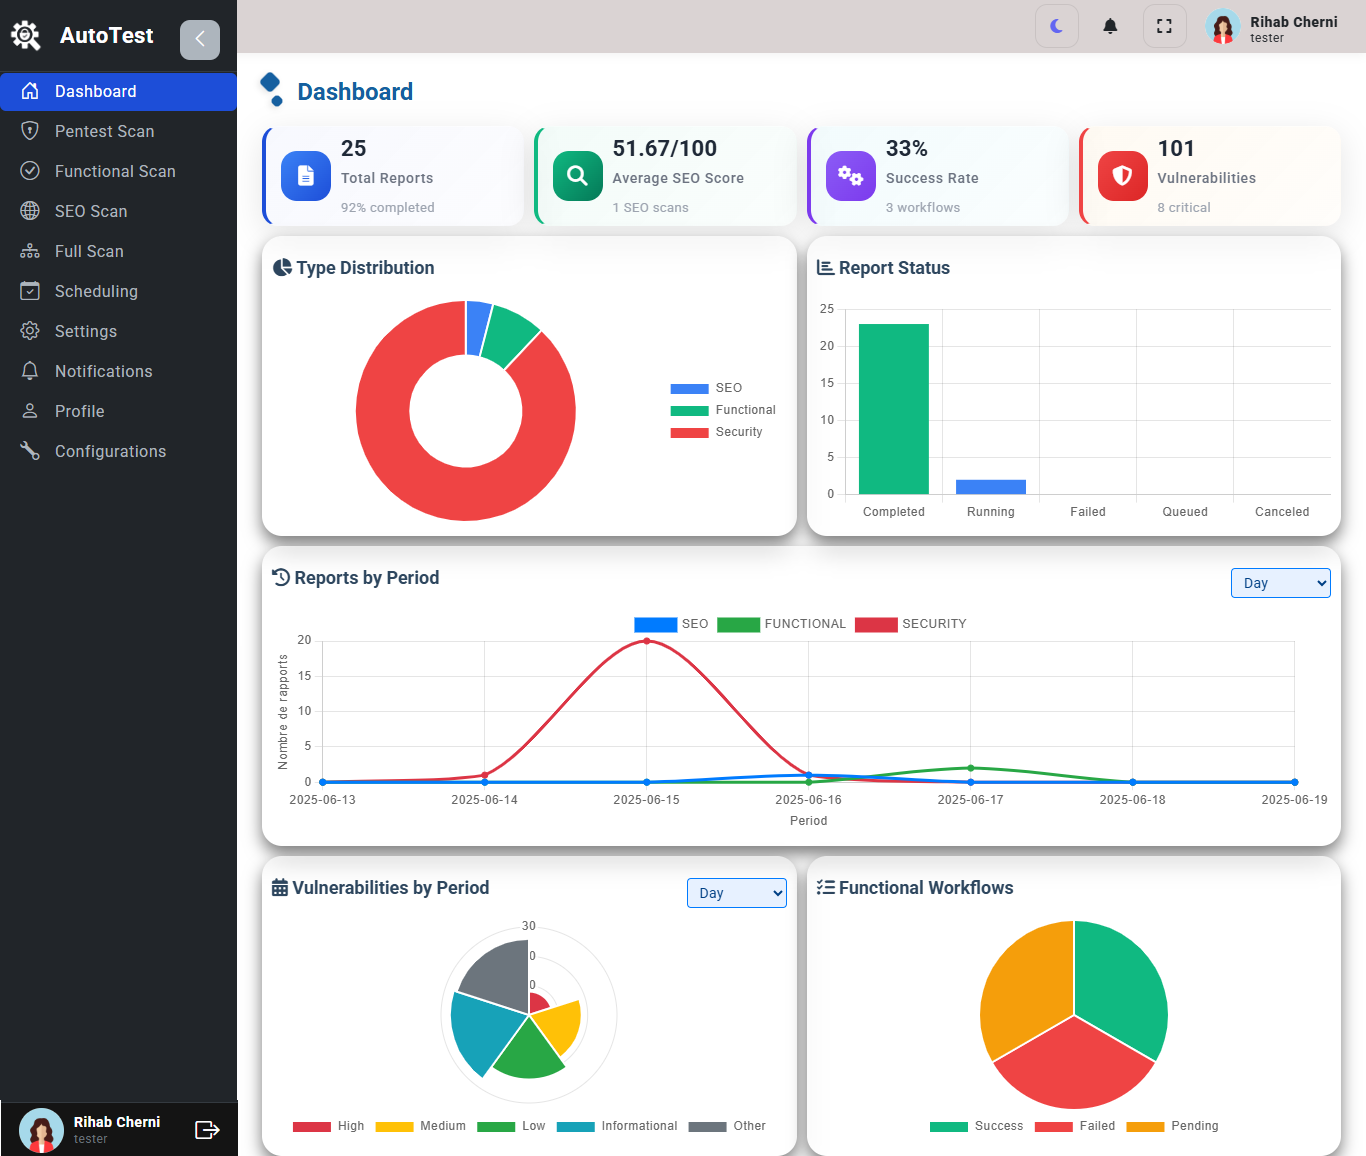
\includegraphics[width=\linewidth]{chapitres/ch4Sp2/section/sprint2.2/img/interface/tester-dashbaord.png}
        \caption{\centering Interface du tableau de bord testeur}
        \label{fig:testerdashboardUI}
    \end{figure}
    \vspace{-0.3cm}

    \item \textbf{Déploiement par conteneurisation} :  
    La figure \ref{fig:deploymentInterfaceUI}\footnote{Voir annexe E : Figure \ref{fig:deploymentInterfaceUI}} illustre le tableau de gestion du déploiement via Docker. Cette interface permet de visualiser le statut de chaque conteneur (backend, frontend, outils de scan), avec la possibilité de redémarrer individuellement les services.
\end{itemize}

